% draft 'Cover Letter'
\documentclass[11pt,apacite]{article}

% packagea for paper
\usepackage{multicol}
\usepackage{flushend}
\usepackage{cite}
\usepackage{longtable}
\usepackage{threeparttable}
\usepackage{amsfonts}
\usepackage{amscd}
\usepackage{hyperref}
\usepackage{times}
\usepackage{paralist}
\usepackage{color}
\usepackage{setspace}
\usepackage{balance}
\usepackage{lastpage}
\usepackage{amsthm}
\usepackage{amsmath}
\usepackage{nomencl}
\usepackage{pstricks}
\usepackage{pstricks-add}
\usepackage{pst-plot,pstricks-add}
\usepackage{lineno}
\usepackage{underscore}
\usepackage{framed}
\usepackage{float}
\usepackage{titlesec}
\usepackage{verbatim}
\usepackage{fancyhdr}
\usepackage{apacite}
\usepackage{filecontents}
\usepackage{natbib}
\usepackage{setspace}
\usepackage{xparse}
\usepackage{booktabs}
\usepackage{graphicx}
\usepackage{subfigure}
\usepackage [english]{babel}
\usepackage [autostyle, english = american]{csquotes}
\usepackage{cite}
\usepackage{tikz}
\newcommand*\circled[1]{\tikz[baseline=(char.base)]{
		\node[shape=circle,draw,inner sep=2pt] (char) {#1};}}

\begin{document}

\begin{center}
This is the \LaTeX  assignment written by Ali Akbar Khan Mohammadi,\\ Introduction to Automata Theory, Formal Languages and Computation,\\ pages 89-92
\end{center}

\begin{center}
\begin{tabular}{clc}  
	\toprule
	\multicolumn{3}{r}{Next State} \\
	\cmidrule(r){2-3}
	Present State    & a & b \\
	\midrule
	\{A\}      & \{B, E\}   & \{B, E\}      \\
	\{B, E\} & \{C, D, F, G\}     & \{C, D, F, G\}      \\
	 \{C, D, F, G\}        & \{H, I\}     & \{H, I\}    \\
	\{H, I\}        & \{H, I\}      & \{H, I\}      \\
	\bottomrule
\end{tabular}
\end{center}	
q$_0^\prime$ : 	\{A\}\\
F$^\prime$ : 	\{C, D, F, G\}\\

Example 3.28: Minimize the following finite automata by the Myhill±Nerode theorem.\\

\begin{center}
	\begin{tabular}{clc}  
		\toprule
		\multicolumn{3}{r}{Next State} \\
		\cmidrule(r){2-3}
		Present State    & I/P= a & I/P= b \\
		\midrule
	  → A     & B  & F     \\
		B & A    & F      \\
		C        & G    & A   \\
		D        & H     & B      \\
		E 		 & A    & G      \\
		F        & H   & C   \\
		G        & A   & D   \\
		H        & A     & C      \\
		\bottomrule
	\end{tabular}
\end{center}
Here F, G, H are final states.\\

\emph{\textbf{Solution:}}

\emph{\textbf{Step I:}} Divide the states of the DFA into two subsets: fi nal (F) and non-final (Q-F).\\
\begin{center}
	F=  \{E, F, G\}, Q-F =  \{A, B, C, D\}
\end{center}
Make a two-dimensional matrix (Fig. 3.53) labelled at the left and bottom by the states of the DFA.
\begin{figure}[H]
	\begin{center}
		\begin{center}
		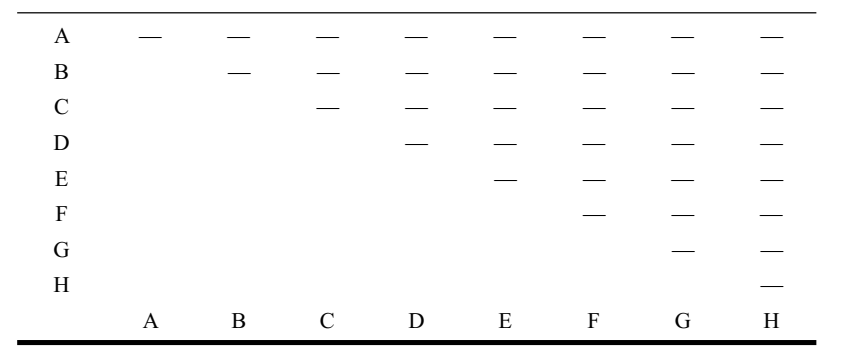
\includegraphics[scale=.45]{Fig353.png}
		\end{center}
		\caption{Fig. 3.53}
	\end{center}
\end{figure}
\emph{\textbf{Step II:}}

\begin{enumerate}
	\item The following combinations are the combination of the beginning and final states.
	\begin{center}
	(A, E), (A, F), (A, G), (B, E), (B, F), (B, G), (C, E), (C, F), (C, G), (D, E), (D, F), (D, G) 
	\end{center}
	Put X in these combinations of states. The modified matrix is given in Fig. 3.54.
	\begin{figure}[H]
		\begin{center}
			\begin{center}
				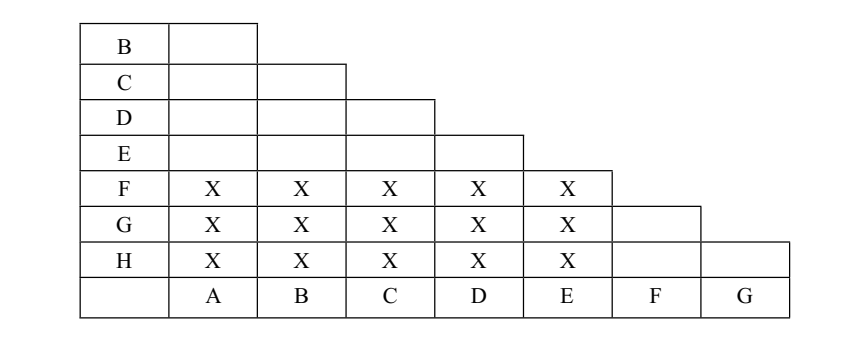
\includegraphics[scale=.45]{Fig354.png}
			\end{center}
			\caption{Fig. 3.54}
		\end{center}
	\end{figure}

		\item The pair combination of non-final states are (A, B), (A, C), (A, D), (A, E), (B, C), (B, D), (B, E), (C, D), (C, E), and (D, E).
		
		r= $\delta$(A, a) → B s = $\delta$(B, a) → A, in the place of (A, B), there is neither X nor x. So, in the place
		of (A, B), there will be 0.
		 
		 Similarly,
		 
		 (r, s) = $\delta$((A, C), a) → (B, G) (there is X). In the place of (A, C), there will be x.\\
		 (r, s) = $\delta$((A, D), a) → (B, H) (there is X). In the place of (A, D), there will be x.\\
		 (r, s) = $\delta$((A, E), a) → (B, A) (there is neither X nor x). In the place of (A, E), there will
		 be 0.\\
		 (r, s) = $\delta$((B, C), a) → (A, G) (there is X). In the place of (B, C), there will be x.\\
		 (r, s) = $\delta$((B, D), a) → (A, H) (there is X). In the place of (B, D), there will be x.\\
		 (r, s) = $\delta$((B, E), a) → (A, A) (there is neither X nor x, only dash). In the place of (B, E),
		 there will be 0.\\
		 (r, s) = $\delta$((C, D), a) → (G, H) (there is neither X nor x). In the place of (C, D), there will
		 be 0.\\
		 (r, s) = $\delta$((C, E), a) → (G, A) (there is X). In the place of (C, E), there will be x.\\
		 (r, s) = $\delta$((D, E), a) → (H, A) (there is X). In the place of (D, E), there will be x.\\
		 
		 \item The pair of combinations of final states are (F, G), (F, H), and (G, H).\\
		 (r, s) = $\delta$((F, G), a) → (A, H) (there is X). In the place of (F, G), there will be x.\\
		 (r, s) = $\delta$((F, H), a) → (H, A) (there is X). In the place of (F, H), there will be x.\\
		 (r, s) = $\delta$((G, H), a) → (A, A) (there is neither X nor x, there is only dash). In the
		 place of (G, H), there will be 0.\\
		 
		 The modified table is given in Fig. 3.55.\\
		 
		 	\begin{figure}[H]
		 	\begin{center}
		 		\begin{center}
		 			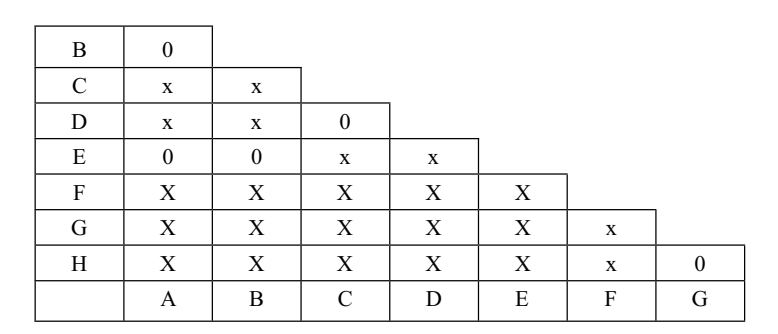
\includegraphics[scale=.45]{Fig355.png}
		 		\end{center}
		 		\caption{Fig. 3.55}
		 	\end{center}
		 \end{figure}
		 
\end{enumerate}

The combination of entries 0 are the states of the modified machine. The states of the minimized
machine are (A, B), (A, E), (B, E), (C, D), (G, H), i.e., (A, B, E), (C, D), (G, H), and (F) (As F is
a final state of the machine, it is left in the state combinations).

(A, B, E) for input µa¶ gives the output (A, B, A) and for input µb¶ gives the output (F, F, G),
where (F, F) belongs to one set and (G) belongs to another set. So, it will be divided into (A, B), (E).
The states of the minimized machines are (A, B),(E), (C, D), (G, H), and (F). Let us name them
as S$_1$, S$_2$, S$_3$, S$_4$, and S$_5$.

For the minimized machine M$^\prime$,

\begin{center}
	Q = \{S$_1$, S$_2$, S$_3$, S$_4$, and S$_5$\}\\
	$\Sigma$ = \{a, b\}
\end{center}

State Table (transitional function $\delta$)


\begin{center}
	\begin{tabular}{clc}  
		\toprule
		\multicolumn{3}{r}{Next State} \\
		\cmidrule(r){2-3}
		Present State    & a & b \\
		\midrule
		S$_1$        & S$_1$    & S$_5$     \\
		S$_2$        & S$_1$    & S$_4$      \\
		S$_3$        & S$_4$    & S$_1$   \\
		S$_4$        & S$_1$    & S$_3$      \\
		S$_5$ 		 & S$_4$    & S$_3$      \\
		\bottomrule
	\end{tabular}
\end{center}

\textbf{3.16 Two-way Finite Automata}\\

Till now, we have studied automata where the reading head moves only in one direction, from left to
right.

\emph{Two-way finite automata} are machines which can traverse (read) an input string in both directions
(left and right).

A two-way DFA (2DFA) consists of five touples M = \{Q, $\Sigma$, $\delta$, q$_0$, F\} where Q, $\Sigma$, q$_0$, and F are defined like one-way FDA,but here the transitional function $\sigma$ is a map from Q × $\Sigma$ to Q × (L, R). L means left
and R means right. Block diagram of a two-way finite automata is shown in Fig. 3.56.\\
\begin{figure}[H]
	\begin{center}
		\begin{center}
			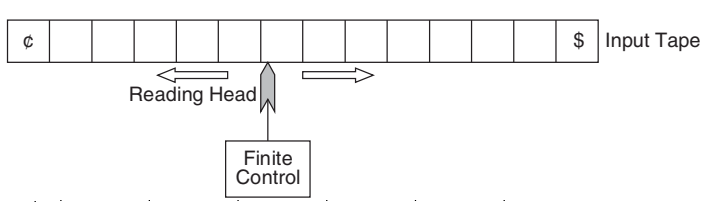
\includegraphics[scale=.45]{Fig356.png}
		\end{center}
		\caption{Fig. 3.56: \emph{Two-way finite automata}}
	\end{center}
\end{figure}
Consider the following example of a two-way DFA; M is given in the following table.\\

\begin{center}
	\begin{tabular}{clc}  
		\toprule
		\multicolumn{3}{r}{Next State} \\
		\cmidrule(r){2-3}
		Present State    & a & b \\
		\midrule
	 → A        & A, R    & B, R     \\
		\circled B       & B, R   & C, L     \\
		C       & A, R    & C, L   \\
		\bottomrule
	\end{tabular}
\end{center}

Let us give a string 101001 to check whether it is accepted by the 2DFA or not.
\begin{center}
(A, 101001)→ (B, 01001R) → (B, 1001R) → (C, 01001L) → (A, 1001R) → (B, 001R) →
(B, 01R)→ (B, 1R) → (C, 01L) → (A, 1R) → B
\end{center}
We have reached the fi nal state, and the string is finished. So, the string 101001 is accepted by the 2DFA.\\

\textbf{3.17 Applications of Finite Automata}\\

Finite automata can be applied in different fi elds of computer science and in different engineering fields.
Some of them are spelling checkers and advisers, multilanguage dictionaries, minimal perfect hashing,
and text compression. Perhaps, the most traditional application is found in compiler construction where
such automata can be used to model and implement efficient lexical analysers.
A typical example is given in Fig. 3.57 (transitional diagram for relational operators in C).

\begin{figure}[H]
	\begin{center}
		\begin{center}
			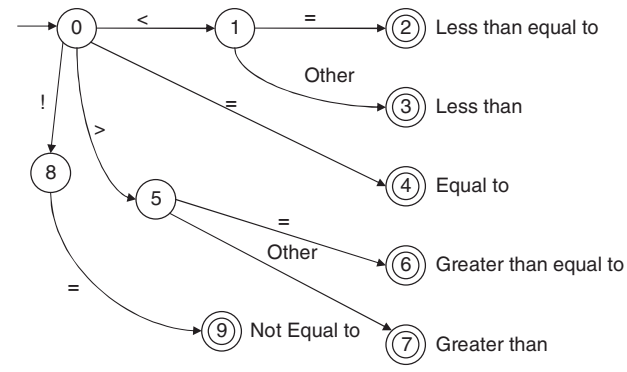
\includegraphics[scale=.45]{Fig357.png}
		\end{center}
		\caption{Fig. 3.57: \emph{Transitional Diagram for Relational Operators in C.}}
	\end{center}
\end{figure}
(\emph{Source}: ``Compilers: Principles, Techniques and tools" Aho, Sethi, Ullman, Pearson Education.)








\end{document}





